\paragraph{}
Une fois le cahier des charges mis en place et l'accord des clients donnés, la première étape du projet consistait à réfléchir au diagramme de Gantt prévisionnel pour les trois mois destinés à la réalisation du projet.
La priorité était donnée aux algorithmes de réalisation des différents rendus espérés grâce au logiciel, et plus particulièrement aux anaglyphes et aux autostéréogrammes. Il fallait revenir sur les algorithmes choisis et présentés dans le cahier des charges, approfondir les recherches pour être sûr de ne passer à côté d'aucun autre algorithme plus performant, et s'approprier le fonctionnement des algorithmes pour les comprendre puis les retranscrire.
En parallèle, d'autres personnes pouvaient travailler sur une partie plus proche du logiciel finale, à savoir la manipulation de la scène ou encore les parseurs de fichiers pour le chargement des objets.
Une fois les manipulations premières de la scène effectuées, les travaux prioritaires seraient le chargement et la sauvegarde de la scène grâce à des fichiers d'extension XML, la création de prises de vue simples ou de folioscopes à partir de la scène et leur sauvegarde, et enfin l'assemblage complet du logiciel avec une interface d'utilisation permettant d'utiliser les différents modules.

\paragraph{}
Un récapitulatif du diagramme de Gantt prévisionnel du projet est donné page suivante.

\newpage
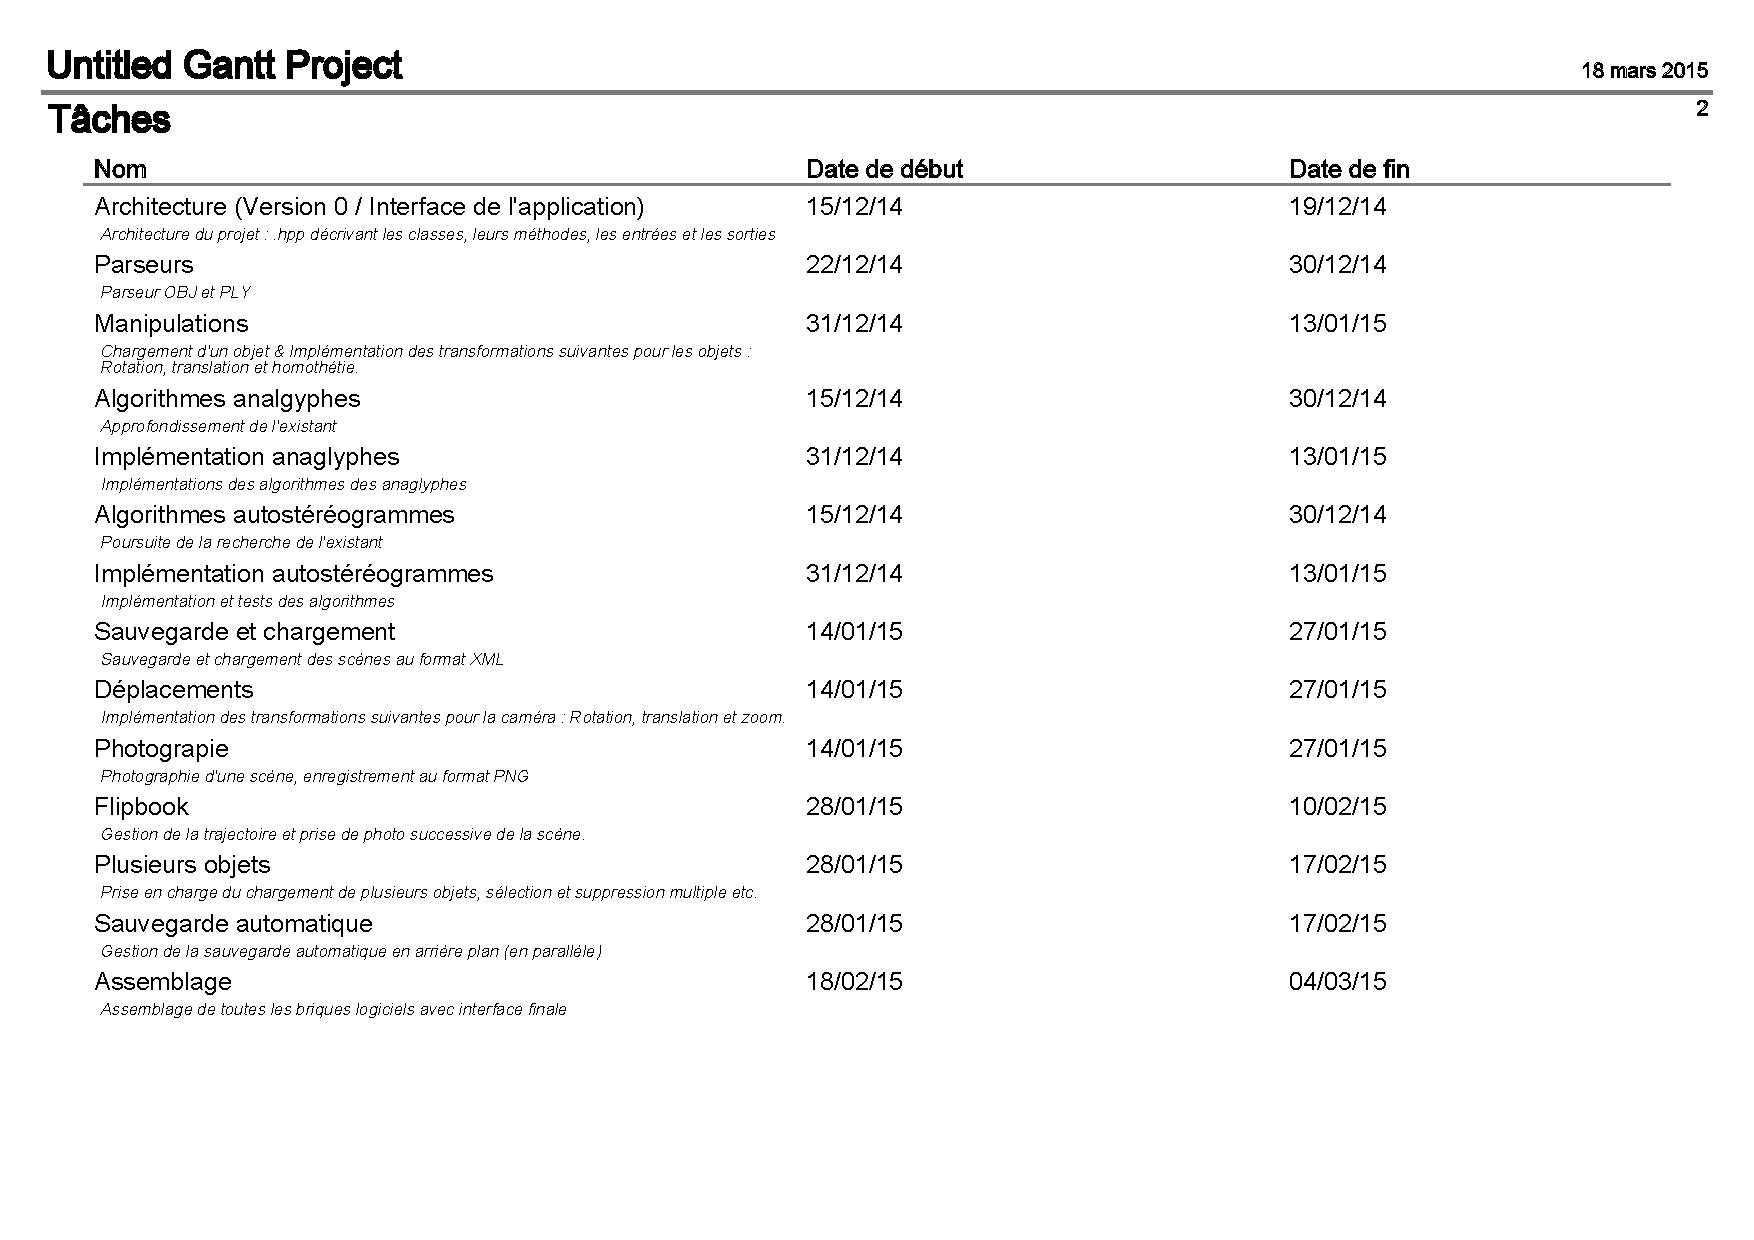
\includepdf[pages=1-1]{gantp.pdf}
\newpage

\paragraph{}
Pour déterminer les durées nécessaires à chaque partie de ce projet, nous avons dû réfléchir aux éventuelles recherches à réaliser au préalable, ainsi qu'à la complexité des tâches en les découpant en sous-parties. Nous avons également réfléchi aux éventuels examens qui auraient pu nous ralentir dans la réalisation en fonction des périodes.

\paragraph{}
Ainsi, pour une tâche telle que l'implémentation d'algorithme d'anaglyphes, il fallait dans un premier temps revenir et compléter les recherches faites sur l'état de l'existant. En effet, comme nous l'avons vu dans la partie présentation du projet, de nombreuses études ont été effectuées pour mettre en place des algorithmes plus ou moins performants capables de générer des anaglyphes. Une fois le choix des algorithmes effectués, l'implémentation de celui-ci en C++ pourrait être effectuée.
Au final, la période déterminée pour la recherche d'algorithmes et l'implémentation de ces algorithmes était d'environ un mois pour une équipe de deux personnes.

\paragraph{}
Un autre exemple de période déterminée est celle destinée à la sauvegarde et au chargement des scènes. Nous avions d'ores et déjà un fichier XML modèle sur lequel s'appuyer, ce qui a permis de passer rapidement à l'implémentation. La sauvegarde consistant simplement en une écriture dans un fichier, seul le chargement demandait des recherches pour déterminer la meilleure bibliothèque pour effectuer le découpage d'un fichier XML. La période déterminée pour cette tâche était de deux semaines pour une équipe de deux personnes.
